\documentclass{article}
%\VignetteIndexEntry{Examples for enhanced mle code}
%\VignettePackage{bbmle}
%\VignetteDepends{aod}
%\VignetteDepends{Hmisc}
%\VignetteDepends{emdbook}
\usepackage[utf8]{inputenc} % for UTF-8/single quotes from sQuote()
\usepackage{graphicx}
\usepackage{natbib}
\usepackage{array}
\usepackage{color}
\usepackage[colorlinks=true,urlcolor=blue,bookmarks=true]{hyperref}
\usepackage{url}
\author{Ben Bolker}
\title{Maximum likelihood estimation and analysis
  with the \code{bbmle} package}
\newcommand{\code}[1]{{\tt #1}}
\date{\today}
\usepackage{Sweave}
\begin{document}
\bibliographystyle{chicago}
%\bibliographystyle{plain}
\maketitle
\tableofcontents



\emph{Note: I have suppressed the continuation character (+) in
  the R examples throughout this document, 
  as I find it easier to read/cut-and-paste where
  necessary.}

The \code{bbmle} package, designed to simplify
maximum likelihood estimation and analysis in R,
extends and modifies the \code{mle} function and class
in the \code{stats4} package that comes with R by default.
\code{mle} is in turn a wrapper around the \code{optim}
function in base R.
The maximum-likelihood-estimation function and class
in \code{bbmle} are both called \code{mle2}, to avoid
confusion and conflict with the original functions in
the \code{stats4} package.  The major differences between
\code{mle} and \code{mle2} are:
\begin{itemize}
\item \code{mle2} is slightly
   more robust, with additional warnings (e.g.
  if the Hessian can't be computed by finite differences,
  \code{mle2} returns a fit with a missing Hessian rather
  than stopping with an error)
\item \code{mle2} uses a \code{data} argument to allow different
  data to be passed to the negative log-likelihood function
\item \code{mle2} has a formula interface like that
 of (e.g.) \code{gls} in the \code{nlme} package.
  For relatively simple models the formula for the
  maximum likelihood can be written in-line, rather than
  defining a negative log-likelihood function.  The formula
  interface also simplifies fitting models with
  categorical variables.  Models fitted using the formula interface
  also have applicable \code{predict} and \code{simulate} methods.
\item \code{bbmle} defines \code{anova}, \code{AIC}, \code{AICc}, 
  and \code{BIC} methods for
  \code{mle2} objects, as well as
  \code{AICtab}, \code{BICtab}, \code{AICctab}
  functions for producing summary tables of information criteria for a 
  set of models.
\end{itemize}

Other packages with similar functionality (extending
GLMs in various ways) are \code{aod} and \code{vgam} (on CRAN), 
\code{gnlr} and \code{gnlr3} in Jim Lindsey's \code{gnlm} package
(\url{http://popgen.unimaas.nl/~jlindsey/rcode.html}).

\section{Example}

This example will use the classic data set on
\emph{Orobanche} germination from \cite{Crowder1978}
(you can also use
\code{glm(...,family="quasibinomial")} or
the \code{aod} package to analyze these data).

\subsection{Test basic fit to simulated beta-binomial data}

First, generate a single beta-binomially distributed
set of points as a simple test.

Load the \code{emdbook} package
to get functions for the beta-binomial distribution (random-deviate 
function \code{rbetabinom} --- these functions are also available
in Jim Lindsey's \code{rmutil} package).
\begin{Schunk}
\begin{Sinput}
> library(emdbook)
\end{Sinput}
\end{Schunk}

Generate random deviates from a random beta-binomial:
\begin{Schunk}
\begin{Sinput}
> set.seed(1001)
> x1 = rbetabinom(n=1000,prob=0.1,size=50,theta=10)
\end{Sinput}
\end{Schunk}

Load the package:
\begin{Schunk}
\begin{Sinput}
> library(bbmle)
\end{Sinput}
\end{Schunk}

Construct a simple negative log-likelihood function:
\begin{Schunk}
\begin{Sinput}
> mtmp <- function(prob,size,theta) {
   -sum(dbetabinom(x1,prob,size,theta,log=TRUE))
 }
\end{Sinput}
\end{Schunk}

Fit the model --- use \code{data} to pass the \code{size}
parameter (since it wasn't hard-coded in the \code{mtmp}
function):
\begin{Schunk}
\begin{Sinput}
> (m0 <- mle2(mtmp,start=list(prob=0.2,theta=9),data=list(size=50)))
\end{Sinput}
\begin{Soutput}
Call:
mle2(minuslogl = mtmp, start = list(prob = 0.2, theta = 9), data = list(size = 50))

Coefficients:
      prob      theta 
 0.1030974 10.0758090 

Log-likelihood: -2723.5 
\end{Soutput}
\end{Schunk}

The \code{summary} method for \code{mle2} objects
shows the parameters; approximate standard
errors (based on quadratic approximation to the curvature at
the maximum likelihood estimate); and a test
of the parameter difference from zero based on
this standard error and on an assumption of normality.

\begin{Schunk}
\begin{Sinput}
> summary(m0)
\end{Sinput}
\begin{Soutput}
Maximum likelihood estimation

Call:
mle2(minuslogl = mtmp, start = list(prob = 0.2, theta = 9), data = list(size = 50))

Coefficients:
        Estimate Std. Error z value     Pr(z)    
prob   0.1030974  0.0031626  32.599 < 2.2e-16 ***
theta 10.0758090  0.6213319  16.216 < 2.2e-16 ***
---
Signif. codes:  0 ‘***’ 0.001 ‘**’ 0.01 ‘*’ 0.05 ‘.’ 0.1 ‘ ’ 1 

-2 log L: 5446.995 
\end{Soutput}
\end{Schunk}

Construct the likelihood profile (you can
apply \code{confint} directly to \code{m0},
but if you're going to work with the likelihood
profile (e.g. plotting, or looking for confidence
intervals at several different $\alpha$ values)
then it is more efficient to compute the profile
once):

\begin{Schunk}
\begin{Sinput}
> p0 <- profile(m0)
\end{Sinput}
\end{Schunk}

Compare the confidence interval estimates based on
inverting a spline fit to the profile (the default);
based on the quadratic approximation at the
maximum likelihood estimate; and based on
root-finding to find the exact point where the
profile crosses the critical level.

\begin{Schunk}
\begin{Sinput}
> confint(p0)
\end{Sinput}
\begin{Soutput}
           2.5 %     97.5 %
prob  0.09709228  0.1095103
theta 8.91708205 11.3559592
\end{Soutput}
\begin{Sinput}
> confint(m0,method="quad")
\end{Sinput}
\begin{Soutput}
           2.5 %     97.5 %
prob  0.09689875  0.1092961
theta 8.85802088 11.2935972
\end{Soutput}
\begin{Sinput}
> confint(m0,method="uniroot")
\end{Sinput}
\begin{Soutput}
           2.5 %     97.5 %
prob  0.09709185  0.1095099
theta 8.91691019 11.3559746
\end{Soutput}
\end{Schunk}

All three types of confidence limits are similar.

Plot the profiles:
\begin{Schunk}
\begin{Sinput}
> par(mfrow=c(1,2))
> plot(p0,plot.confstr=TRUE)
\end{Sinput}
\end{Schunk}
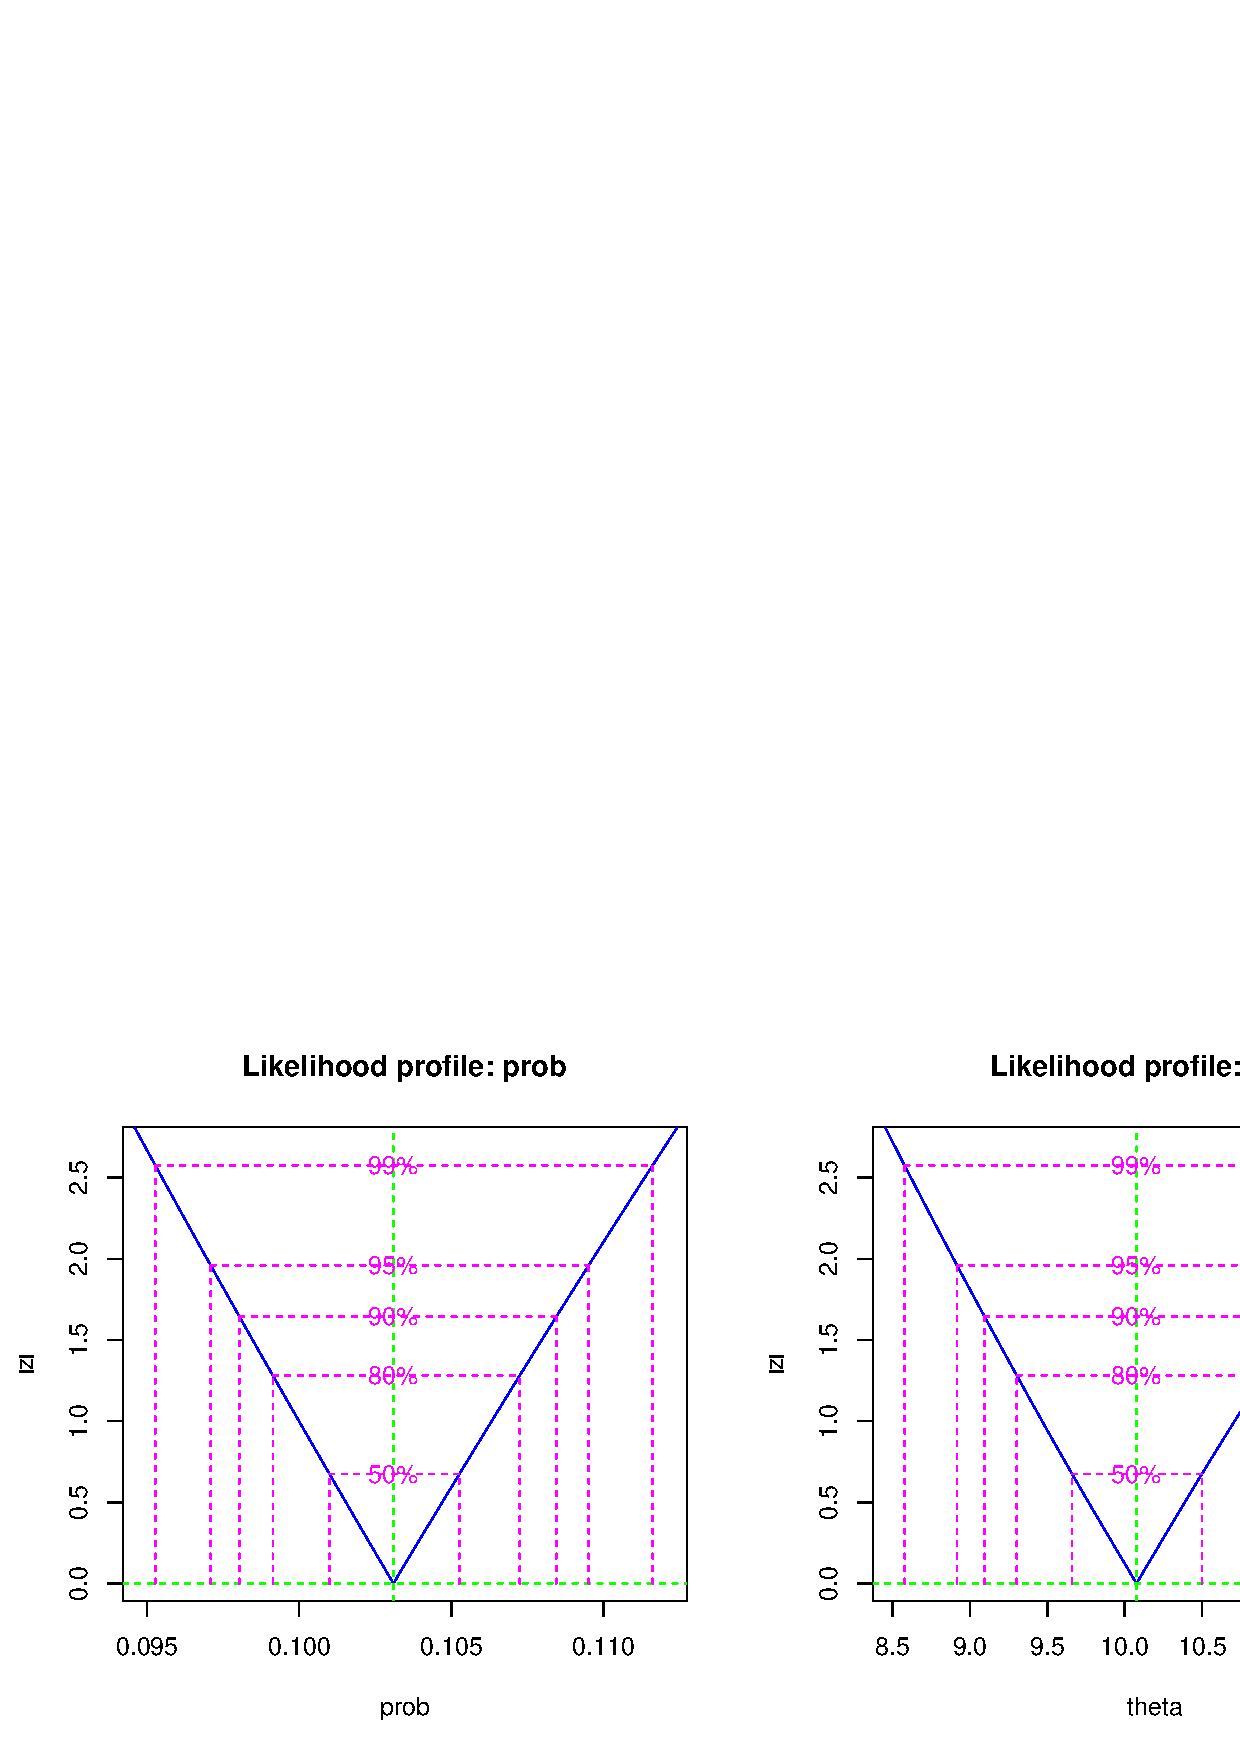
\includegraphics{mle2-profplot1}

By default, the plot method for 
likelihood profiles displays the square root of the
the deviance
(twice the difference in negative
log-likelihood), so it will
be {\sf V}-shaped
for cases where the quadratic approximation works well
(as in this case).
(For a better visual estimate of whether the profile
is quadratic, use the \code{absVal=FALSE} option to the \code{plot}
method.)

You can also request confidence intervals
calculated using \code{uniroot}, which may be more exact when
the profile is not smooth enough to be modeled accurately
by a spline.  However, this method is
also more sensitive to numeric problems.

Instead of defining an
explicit function for \code{minuslogl}, 
we can also use the formula interface.
The formula interface assumes that
the density function given (1) has \code{x} as
its first argument (if the distribution is multivariate,
then \code{x} should be a matrix of observations)
and (2) has a \code{log} argument that will return
the log-probability or log-probability density
if \code{log=TRUE}.
\begin{Schunk}
\begin{Sinput}
> m0f <- mle2(x1~dbetabinom(prob,size=50,theta),
             start=list(prob=0.2,theta=9))
\end{Sinput}
\end{Schunk}

It's convenient to use the formula interface
to try out likelihood estimation on the
transformed parameters:
\begin{Schunk}
\begin{Sinput}
> m0cf <- mle2(x1~dbetabinom(prob=plogis(lprob),size=50,theta=exp(ltheta)),
             start=list(lprob=0,ltheta=2))
> confint(m0cf,method="uniroot")
\end{Sinput}
\begin{Soutput}
           2.5 %    97.5 %
lprob  -2.229963 -2.095757
ltheta  2.187950  2.429744
\end{Soutput}
\begin{Sinput}
> confint(m0cf,method="spline")
\end{Sinput}
\begin{Soutput}
           2.5 %    97.5 %
lprob  -2.229963 -2.095756
ltheta  2.187948  2.429742
\end{Soutput}
\end{Schunk}

In this case the answers from \code{uniroot}
and \code{spline} (default) methods barely
differ.

\subsection{Real data (\emph{Orobanche}, \cite{Crowder1978})}
Data as incorporated in the \code{aod} package:
\begin{Schunk}
\begin{Sinput}
> library(aod)
\end{Sinput}
\begin{Soutput}
Package aod, version 1.1-33 
\end{Soutput}
\begin{Sinput}
> data(orob1)
\end{Sinput}
\end{Schunk}

Now construct a negative log-likelihood
function that differentiates among groups:
\begin{Schunk}
\begin{Sinput}
> ML1 <- function(prob1,prob2,prob3,theta,x) {
   prob <- c(prob1,prob2,prob3)[as.numeric(x$dilution)]
   size <- x$n
   -sum(dbetabinom(x$y,prob,size,theta,log=TRUE))
 }
\end{Sinput}
\end{Schunk}

Results from \cite{Crowder1978}:
% latex.default(crowder.results, file = "", table.env = FALSE,      title = "model") 
%
\begin{center}
 \begin{tabular}{lrrrrrrrr}\hline\hline
\multicolumn{1}{l}{model}&\multicolumn{1}{c}{prob1}&\multicolumn{1}{c}{prob2}&\multicolumn{1}{c}{prob3}&\multicolumn{1}{c}{theta}&\multicolumn{1}{c}{sd.prob1}&\multicolumn{1}{c}{sd.prob2}&\multicolumn{1}{c}{sd.prob3}&\multicolumn{1}{c}{NLL}\tabularnewline
\hline
prop diffs&$0.132$&$0.871$&$0.839$&$78.424$&$0.027$&$0.028$&$0.032$&$-34.991$\tabularnewline
full model&$$&$$&$$&$$&$$&$$&$$&$-34.829$\tabularnewline
homog model&$$&$$&$$&$$&$$&$$&$$&$-56.258$\tabularnewline
\hline
\end{tabular}

\end{center}                            
\begin{Schunk}
\begin{Sinput}
> (m1 <- mle2(ML1,start=list(prob1=0.5,prob2=0.5,prob3=0.5,theta=1),
     data=list(x=orob1)))
\end{Sinput}
\begin{Soutput}
Call:
mle2(minuslogl = ML1, start = list(prob1 = 0.5, prob2 = 0.5, 
    prob3 = 0.5, theta = 1), data = list(x = orob1))

Coefficients:
     prob1      prob2      prob3      theta 
 0.1318187  0.8706259  0.8382504 73.7968323 

Log-likelihood: -34.99 

Warning: optimization did not converge (code 1)
\end{Soutput}
\end{Schunk}

Or:
The result warns us that the optimization has not
converged; we also don't match
Crowder's results for $\theta$ exactly.
We can fix this by setting \code{parscale} appropriately.

\begin{Schunk}
\begin{Sinput}
> (m2 <- mle2(ML1,start=as.list(coef(m1)),
           control=list(parscale=coef(m1)),
           data=list(x=orob1)))
\end{Sinput}
\begin{Soutput}
Call:
mle2(minuslogl = ML1, start = as.list(coef(m1)), data = list(x = orob1), 
    control = list(parscale = coef(m1)))

Coefficients:
     prob1      prob2      prob3      theta 
 0.1322123  0.8708913  0.8393195 78.4227905 

Log-likelihood: -34.99 
\end{Soutput}
\end{Schunk}

Calculate likelihood profile (restrict the upper limit
of $\theta$, simply because it will make the picture
below a little bit nicer):
\begin{Schunk}
\begin{Sinput}
> p2 <- profile(m2,prof.upper=c(Inf,Inf,Inf,theta=2000))
\end{Sinput}
\end{Schunk}

Get the curvature-based parameter standard
deviations (which Crowder used
rather than computing likelihood profiles):
\begin{Schunk}
\begin{Sinput}
> round(sqrt(diag(vcov(m2))),3)
\end{Sinput}
\begin{Soutput}
 prob1  prob2  prob3  theta 
 0.028  0.029  0.032 74.238 
\end{Soutput}
\end{Schunk}
We are slightly off Crowder's numbers --- rounding
error?

Crowder also defines a variance (overdispersion) parameter
$\sigma^2=1/(1+\theta)$.
\begin{Schunk}
\begin{Sinput}
> sqrt(1/(1+coef(m2)["theta"]))
\end{Sinput}
\begin{Soutput}
    theta 
0.1122089 
\end{Soutput}
\end{Schunk}

Using the delta method (via the \code{deltavar}
function in the \code{emdbook} package)
to approximate the standard deviation of
$\sigma$:
\begin{Schunk}
\begin{Sinput}
> sqrt(deltavar(sqrt(1/(1+theta)),meanval=coef(m2)["theta"],
          vars="theta",Sigma=vcov(m2)[4,4]))
\end{Sinput}
\begin{Soutput}
[1] 0.05244185
\end{Soutput}
\end{Schunk}

Another way to fit in terms of $\sigma$ rather than $\theta$
is to compute $\theta=1/\sigma^2-1$ on the fly in a
formula:

\begin{Schunk}
\begin{Sinput}
> m2b <- mle2(y~dbetabinom(prob,size=n,theta=1/sigma^2-1),
             data=orob1,
             parameters=list(prob~dilution,sigma~1),
             start=list(prob=0.5,sigma=0.1))
> round(sqrt(diag(vcov(m2b))),3)["sigma"]
\end{Sinput}
\begin{Soutput}
sigma 
0.052 
\end{Soutput}
\begin{Sinput}
> p2b <- profile(m2b,prof.lower=c(-Inf,-Inf,-Inf,0))
\end{Sinput}
\end{Schunk}

As might be expected since the standard deviation
of $\sigma$ is large, the quadratic approximation is
poor:

\begin{Schunk}
\begin{Sinput}
> r1 <- rbind(confint(p2)["theta",],
             confint(m2,method="quad")["theta",])
> rownames(r1) <- c("spline","quad")
> r1
\end{Sinput}
\begin{Soutput}
           2.5 %   97.5 %
spline  19.67166       NA
quad   -67.08083 223.9264
\end{Soutput}
\end{Schunk}

Plot the profile:
\begin{Schunk}
\begin{Sinput}
> plot(p2,which="theta",plot.confstr=TRUE)
\end{Sinput}
\end{Schunk}
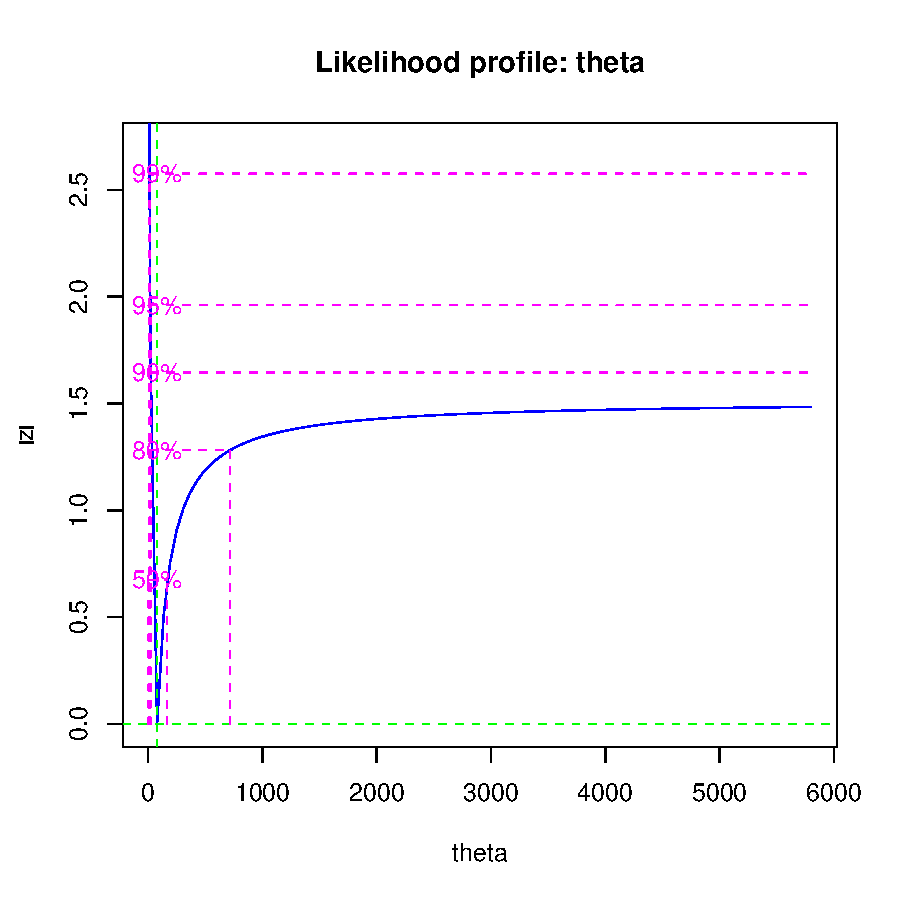
\includegraphics{mle2-025}

What does the profile for $\sigma$ look like?
\begin{Schunk}
\begin{Sinput}
> plot(p2b,which="sigma",plot.confstr=TRUE,
      show.points=TRUE)
\end{Sinput}
\end{Schunk}
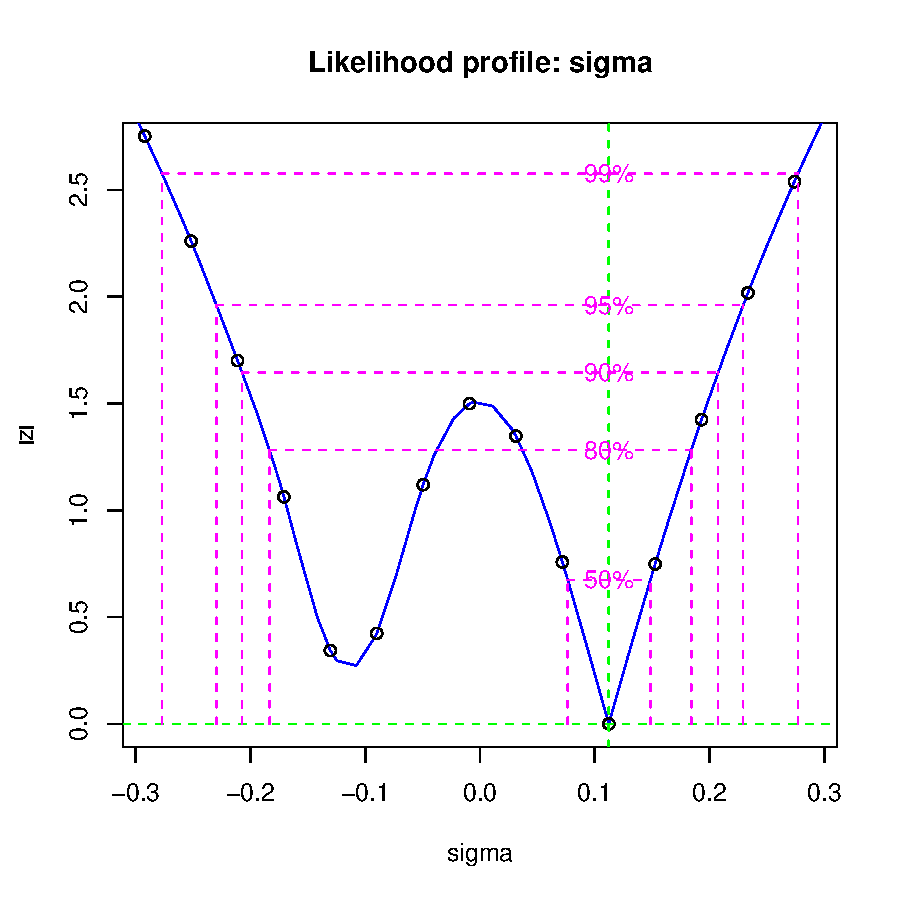
\includegraphics{mle2-026}

Now fit a homogeneous model:
\begin{Schunk}
\begin{Sinput}
> ml0 <- function(prob,theta,x) {
   size <- x$n
   -sum(dbetabinom(x$y,prob,size,theta,log=TRUE))
 }
> m0 <- mle2(ml0,start=list(prob=0.5,theta=100),
           data=list(x=orob1))
\end{Sinput}
\end{Schunk}

The log-likelihood matches Crowder's result:
\begin{Schunk}
\begin{Sinput}
> logLik(m0)
\end{Sinput}
\begin{Soutput}
'log Lik.' -56.25774 (df=2)
\end{Soutput}
\end{Schunk}

It's easier to 
use the formula interface
to specify all three of the models
fitted by Crowder (homogeneous, probabilities differing
by group, probabilities and overdispersion differing
by group):

\begin{Schunk}
\begin{Sinput}
> m0f <- mle2(y~dbetabinom(prob,size=n,theta),
             parameters=list(prob~1,theta~1),
             data=orob1,
             start=list(prob=0.5,theta=100))
> m2f <- mle2(y~dbetabinom(prob,size=n,theta),
             parameters=list(prob~dilution,theta~1),
             data=orob1,
             start=list(prob=0.5,theta=78.424))
> m3f <- mle2(y~dbetabinom(prob,size=n,theta),
             parameters=list(prob~dilution,theta~dilution),
             data=orob1,
             start=list(prob=0.5,theta=78.424))
\end{Sinput}
\end{Schunk}

\code{anova} runs a likelihood ratio test on nested
models:
\begin{Schunk}
\begin{Sinput}
> anova(m0f,m2f,m3f)
\end{Sinput}
\begin{Soutput}
Likelihood Ratio Tests
Model 1: m0f, y~dbetabinom(prob,size=n,theta): prob~1, theta~1
Model 2: m2f, y~dbetabinom(prob,size=n,theta): prob~dilution, theta~1
Model 3: m3f, y~dbetabinom(prob,size=n,theta): prob~dilution,
          theta~dilution
  Tot Df Deviance   Chisq Df Pr(>Chisq)    
1      2  112.515                          
2      4   69.981 42.5341  2  5.805e-10 ***
3      6   69.981  0.0008  2     0.9996    
---
Signif. codes:  0 ‘***’ 0.001 ‘**’ 0.01 ‘*’ 0.05 ‘.’ 0.1 ‘ ’ 1 
\end{Soutput}
\end{Schunk}

The various \code{ICtab} commands produce tables of
information criteria, optionally sorted and
with model weights.
\begin{Schunk}
\begin{Sinput}
> AICtab(m0f,m2f,m3f,weights=TRUE,delta=TRUE,sort=TRUE)
\end{Sinput}
\begin{Soutput}
    dAIC df weight
m2f  0.0 4  0.881 
m3f  4.0 6  0.119 
m0f 38.5 2  <0.001
\end{Soutput}
\begin{Sinput}
> BICtab(m0f,m2f,m3f,delta=TRUE,nobs=nrow(orob1),sort=TRUE,weights=TRUE)
\end{Sinput}
\begin{Soutput}
    dBIC df weight
m2f  0.0 4  0.9412
m3f  5.5 6  0.0588
m0f 37.0 2  <0.001
\end{Soutput}
\begin{Sinput}
> AICctab(m0f,m2f,m3f,delta=TRUE,nobs=nrow(orob1),sort=TRUE,weights=TRUE)
\end{Sinput}
\begin{Soutput}
    dAICc df weight 
m2f  0.0  4  0.99222
m3f  9.7  6  0.00778
m0f 35.8  2  < 0.001
\end{Soutput}
\end{Schunk}

\section*{Additions/enhancements/differences from \code{stats4::mle}}
\begin{itemize}
\item{\code{anova} method}
\item{warnings on convergence failure}
\item{more robust to non-positive-definite Hessian;
  can also specify \code{skip.hessian} to skip Hessian
  computation when it is problematic}
\item{when profiling fails because better value is
    found, report new values}
\item{can take named vectors as well as lists as
    starting parameter vectors}
\item{added \code{AICc}, \code{BIC} definitions,
    \code{ICtab} functions}
\item{added \code{"uniroot"} and \code{"quad"}
    options to \code{confint}}
\item{more options for colors and line types etc etc.
The old arguments are:
\begin{Schunk}
\begin{Sinput}
> function (x, levels, conf = c(99, 95, 90, 80, 50)/100, nseg = 50,
           absVal = TRUE, ...) {}
\end{Sinput}
\end{Schunk}
The new one is:
\begin{Schunk}
\begin{Sinput}
> function (x, levels, which=1:p, conf = c(99, 95, 90, 80, 50)/100, nseg = 50,
           plot.confstr = FALSE, confstr = NULL, absVal = TRUE, add = FALSE,
           col.minval="green", lty.minval=2,
           col.conf="magenta", lty.conf=2,
           col.prof="blue", lty.prof=1,
           xlabs=nm, ylab="score",
           show.points=FALSE,
           main, xlim, ylim, ...) {}
\end{Sinput}
\end{Schunk}
\code{which} selects (by character vector or numbers)
which parameters to plot: \code{nseg} does nothing
(even in the old version); \code{plot.confstr} turns on
the labels for the confidence levels; \code{confstr} gives
the labels; \code{add} specifies whether to add the
profile to an existing plot; \code{col} and \code{lty}
options specify the colors and line types for
horizontal and vertical lines marking the minimum
and confidence vals and the profile curve; \code{xlabs}
gives a vector of x labels; \code{ylab} gives the y label;
\code{show.points} specifies whether to show the raw points
computed.
}
\item{\code{mle.options()}}
\item{\code{data} argument}
\item{handling of names in argument lists}
\item{can use alternative optimizers (\code{nlminb}, \code{constrOptim})}
\end{itemize}




\section{Newer stuff}

\textbf{To do:}
\begin{itemize}
  \item{use \code{predict}, \code{simulate} etc.
    to demonstrate different parametric bootstrap approaches
    to confidence and prediction intervals
    \begin{itemize}
      \item use \code{predict} to get means and standard
        deviations, use delta method?
      \item use \code{vcov}, assuming quadratic profiles,
        with \code{predict(\ldots,newparams=\ldots)}
      \item prediction intervals assuming no parameter uncertainty
        with \code{simulate}
      \item both together \ldots
      \end{itemize}
    }
  \end{itemize}

\section{Example}

Data from an experiment by Vonesh \citep{VoneshBolker2005}
\begin{Schunk}
\begin{Sinput}
> frogdat <- data.frame(
   size=rep(c(9,12,21,25,37),each=3),
   killed=c(0,2,1,3,4,5,rep(0,4),1,rep(0,4)))
> frogdat$initial <- rep(10,nrow(frogdat))
\end{Sinput}
\end{Schunk}

\begin{Schunk}
\begin{Sinput}
> library(ggplot2)
\end{Sinput}
\end{Schunk}

\begin{Schunk}
\begin{Sinput}
> gg1 <- ggplot(frogdat,aes(x=size,y=killed))+geom_point()+
       stat_sum(aes(size=factor(..n..)))+
       labs(size="#")+scale_x_continuous(limits=c(0,40))
\end{Sinput}
\end{Schunk}

\begin{Schunk}
\begin{Sinput}
> m3 <- mle2(killed~dbinom(prob=c*(size/d)^g*exp(1-size/d),
   size=initial),data=frogdat,start=list(c=0.5,d=5,g=1))
> pdat <- data.frame(size=1:40,initial=rep(10,40))
> pdat1 <- data.frame(pdat,killed=predict(m3,newdata=pdat))
\end{Sinput}
\end{Schunk}

\begin{Schunk}
\begin{Sinput}
> m4 <- mle2(killed~dbinom(prob=c*((size/d)*exp(1-size/d))^g,
   size=initial),data=frogdat,start=list(c=0.5,d=5,g=1))
> pdat2 <- data.frame(pdat,killed=predict(m4,newdata=pdat))
\end{Sinput}
\end{Schunk}

\begin{Schunk}
\begin{Sinput}
> print(gg1 + geom_line(data=pdat1,colour="red")+geom_line(data=pdat2,colour="blue"))
\end{Sinput}
\end{Schunk}
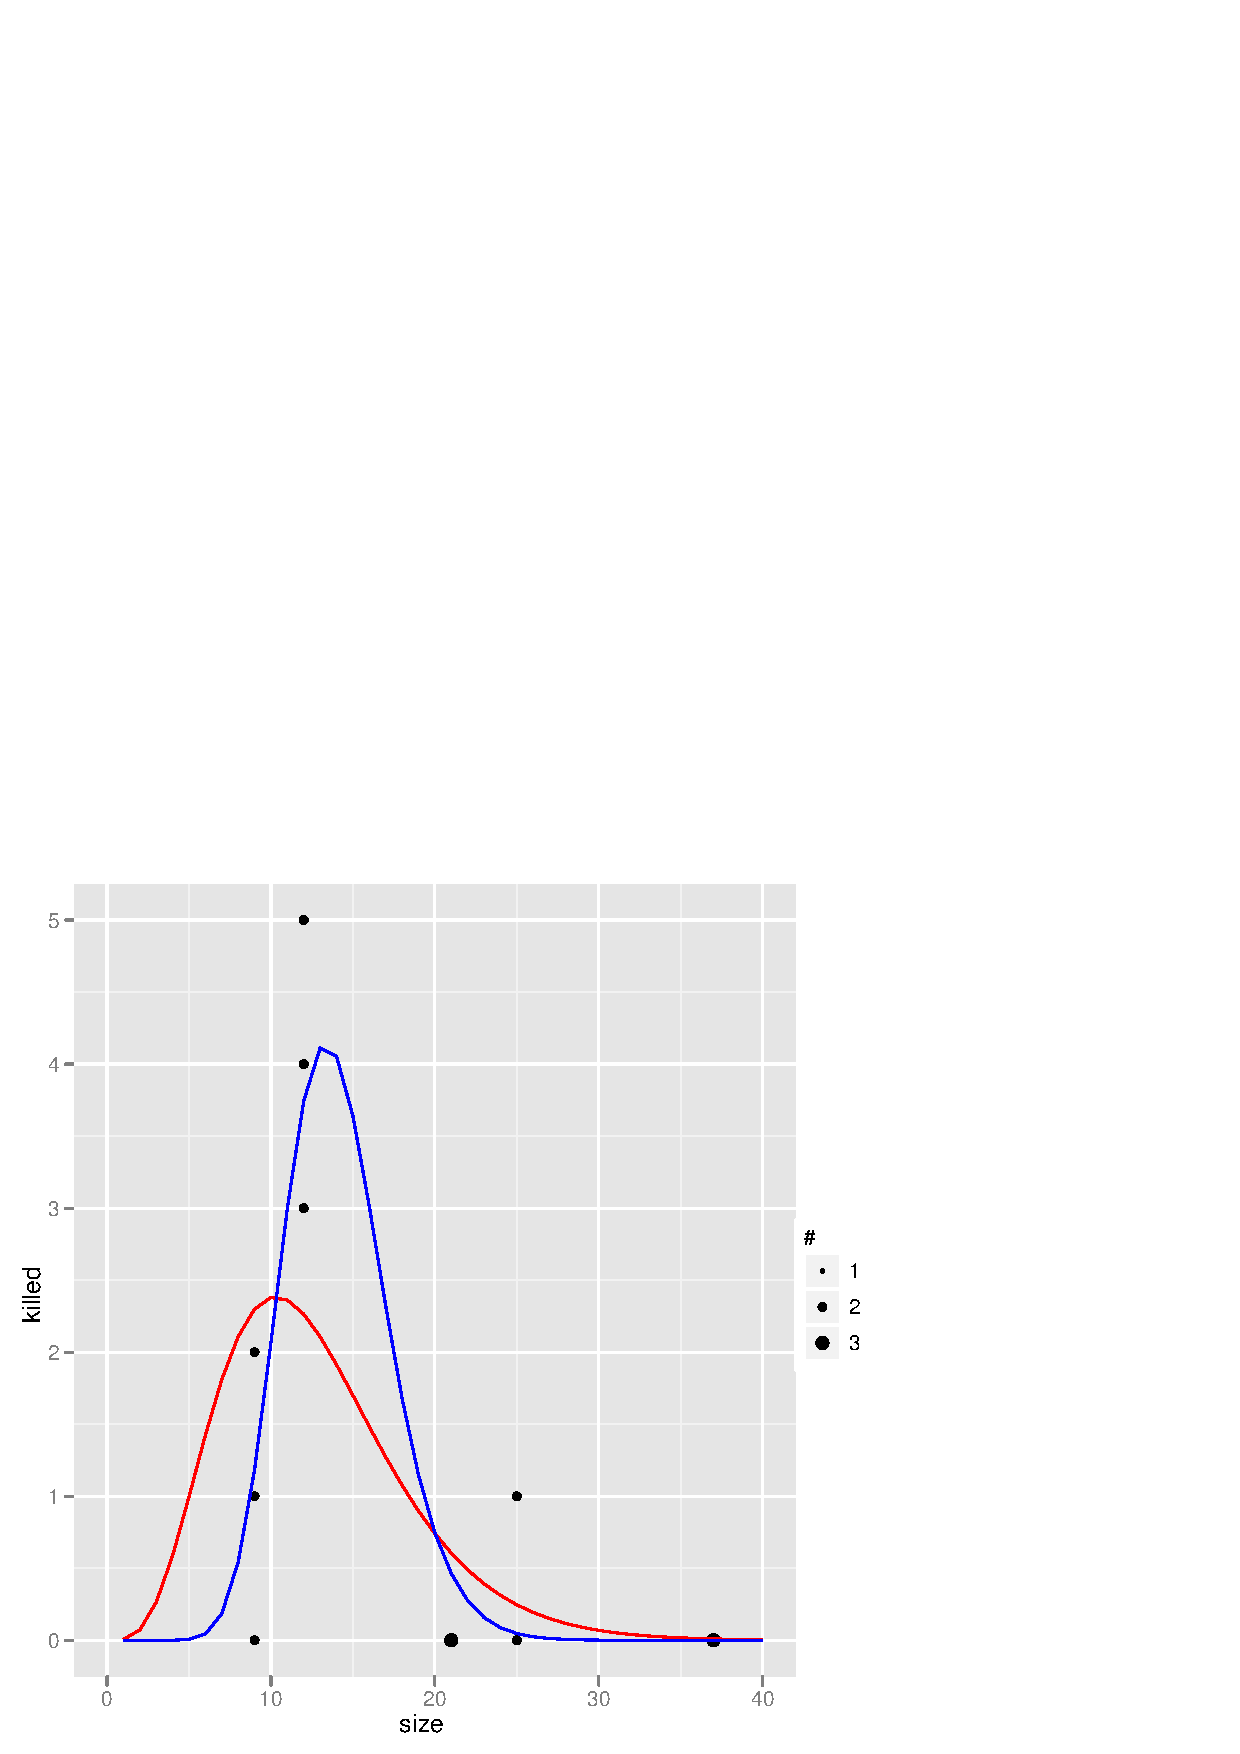
\includegraphics{mle2-039}

\begin{Schunk}
\begin{Sinput}
> coef(m4)
\end{Sinput}
\begin{Soutput}
         c          d          g 
 0.4138847 13.3517574 18.2511264 
\end{Soutput}
\begin{Sinput}
> prof4 <- profile(m4)
\end{Sinput}
\end{Schunk}

Three different ways to draw the profile:
\begin{Schunk}
\begin{Sinput}
> print(plot(prof4))
\end{Sinput}
\begin{Soutput}
NULL
\end{Soutput}
\end{Schunk}

\setkeys{Gin}{width=\textwidth}
\begin{Schunk}
\begin{Sinput}
> prof4_df <- as.data.frame(prof4)
> library(lattice)
> print(xyplot(abs(z)~focal|param,data=prof4_df,
        subset=abs(z)<3,
        type="b",
        xlab="",
        ylab=expression(paste(abs(z),
            " (square root of ",Delta," deviance)")),
        scale=list(x=list(relation="free")),
              layout=c(3,1)))
\end{Sinput}
\end{Schunk}
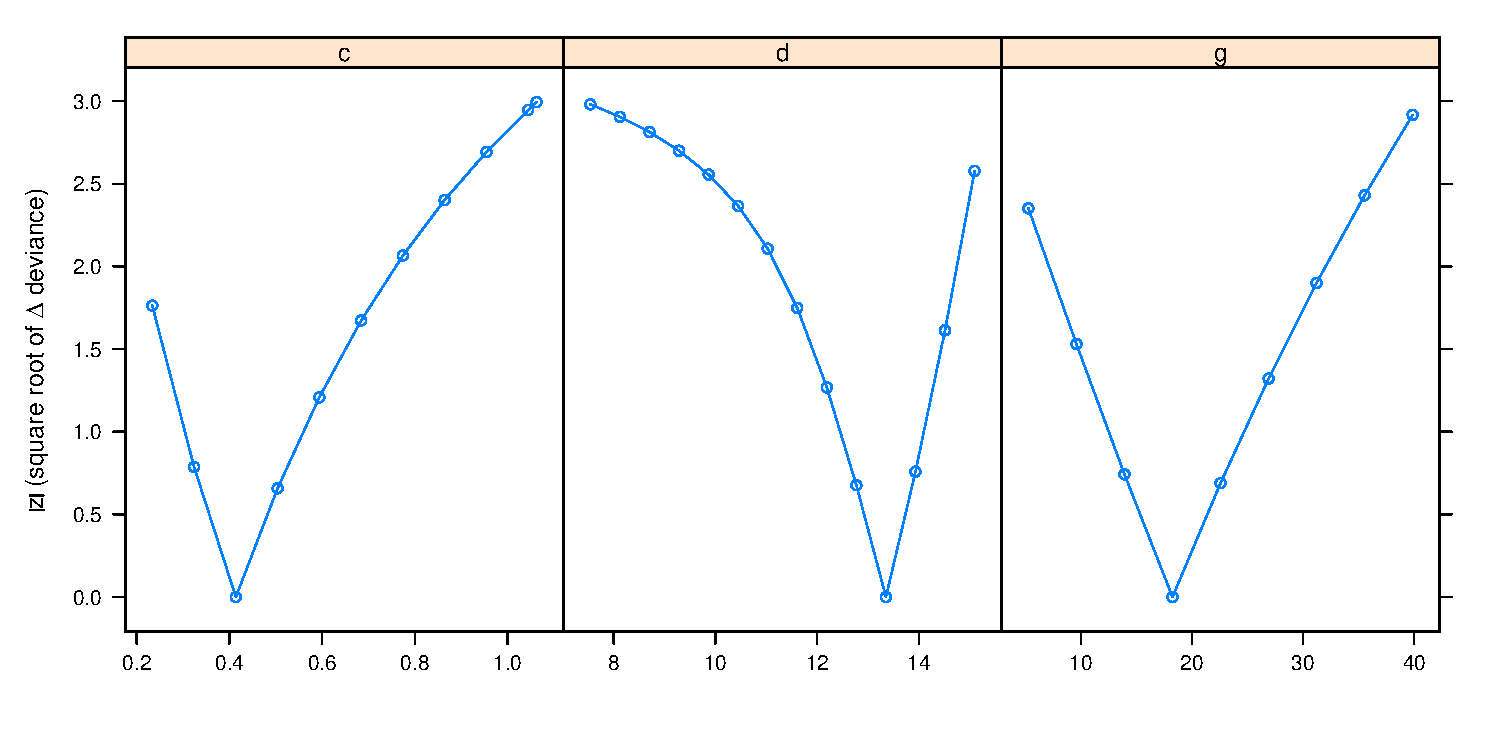
\includegraphics{mle2-latticeprof}

\begin{Schunk}
\begin{Sinput}
> print(ggplot(subset(prof4_df,abs(z)<3),
        aes(x=focal,y=abs(z)))+geom_line()+
       geom_point()+
       facet_grid(~param,scale="free_x"))
\end{Sinput}
\end{Schunk}
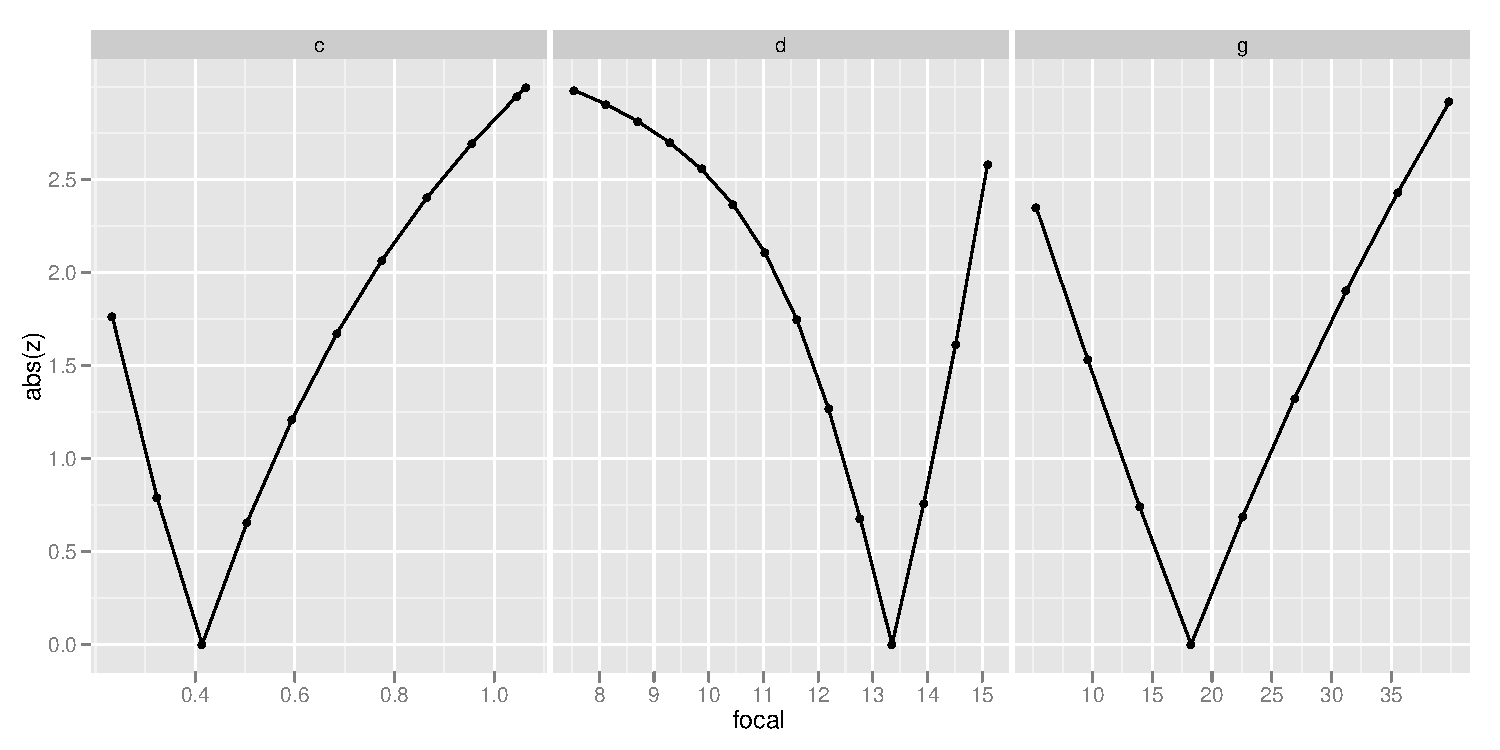
\includegraphics{mle2-ggplotprof}

\section*{Bugs, wishes, to do}
\begin{itemize}
\item \textbf{WISH}: further methods and arguments: \code{subset},
  \code{predict}, \code{resid}: \code{sim}?
\item \textbf{WISH}: extend ICtab to allow DIC as well?
\item minor \textbf{WISH}: 
  better methods for extracting \code{nobs} information
  when possible (e.g. with formula interface)
\item \textbf{WISH}: better documentation, especially for S4 methods
\item \textbf{WISH}: variable-length chunks in argument list
\item \textbf{WISH}: limited automatic differentiation
    (add capability for common distributions)
\end{itemize}

\bibliography{mle2}
\end{document}
